\usetikzlibrary{arrows, calc}

\lstset{basicstyle=\ttfamily,
	language=SQL,
	deletekeywords={NUMBER} % number ist ein Attribut in diesem Blatt
}
\begin{document}
\lecture{Implementierung von Datenbanksystemen}{IDB}
\title{Übungsblatt~10}
\subtitle{Anfrageverarbeitung}
\maketitle

\section*{Lernziele}

\begin{itemize}
  \item Erstellung und algebraische Optimierung von Ausführungsplänen mit Sichten
  \item Optimierung in der Praxis
\end{itemize}

\section*{Literatur}

\HaerderNintyNine{11, 12}

\ElmasriSeventh{18, 19}

\GarciaMolinaSecond{8, 15, 16}

\NeumannFifteen


\section{Fragen zur Vorlesung}

\begin{enumerate}[a)]
	\item Was ist die Aufgabe der Anfrageverarbeitung?

	\begin{solution}
	Abbildung von mengenorientierten Operationen auf effiziente satzorientierte Operationen.
	D.\,h.\ von oben kommen nun keine Satzoperationen mehr, sondern mengenorientierte (Relationenalgebra, SQL).
	Das verringert oft den Programmieraufwand (Beispiel: Mitarbeiter und Abteilungen, VL 10-22).
	Außerdem ist es einfacher zu optimieren.
	Insbesondere muss bei Änderungen an Kardinalitäten etc.\ nicht die Programmstruktur geändert werden.
	Das macht der Optimierer für uns.
	\end{solution}

	\item Aus welchen Schritten besteht sie?

	\begin{note}
	Bild an die Tafel.\\
	Oracle macht das übrigens so 	\url{https://docs.oracle.com/database/121/TGSQL/tgsql_sqlproc.htm\#TGSQL175}
	\end{note}
	\beamertxt{\pagebreak}

	\begin{solution}
	Siehe Folien~\Anfrageverarbeitung.

	Härder:
		Parser macht lexikalische und syntaktische Analyse.
		Semantische Analyse wird bereits mit der Interndarstellung gemacht.
		Das sind Namensauflösung und Typumwandlung.
		Zugriffs- und Integritätskontrolle sind eine Erweiterung der semantischen Analyse.
		"`Standardisierung und Vereinfachung"' und "`Restrukturierung und Transformation"' sind gemeinsam die Optimierung.
	\end{solution}

	\item Angenommen eine Anfrage wird mit gleichen Parametern erneut ausgeführt: Welche Schritte könnten unter welchen Bedingungen eingespart werden?

	\begin{solution}
	Das ist schwieriger, als man denkt:
\begin{itemize}
	\item Sollten sich die Daten nicht geändert haben, könnte man das selbe Ergebnis zurückgeben.
	\item Wenn sich die Daten nur leicht ändern, müsste man nur die Ausführung erneut durchführen, da sich ein anderes Ergebnis ergibt.
	\item Ändern sich die Daten stark, so muss auch die Optimierung erneut durchgeführt werden.
	\item Ändern die Berechtigungen, so muss die Zugriffskontrolle erneut durchgeführt werden.
\end{itemize}
	Rein theoretisch kann man diese Fälle feststellen (Jedes Grant/Revoke prüfen; Statistiken für den Optimierer werden nur explizit geändert, dann kann man prüfen.),
	jedoch wird in der Praxis mit wenigen Ausnahmen einfach die gesamte Anfrageverarbeitung erneut durchgeführt.
	Eine Ausnahme bilden explizit gespeicherte Prozeduren und Funktionen (z.b. PL/SQL).
	\end{solution}

	\item Nun mit unterschiedlichen Parametern.

	\begin{solution}
	Zusätzlich zu den obigen Schritten muss nur die Typkonversion erneut durchgeführt werden.
	Sinnvoll kann zusätzlich eine erneute Optimierung sein ($\mathrm{Wert} > 10$; $\mathrm{Wert} > 1000000$).
	\end{solution}
\end{enumerate}
\begin{beamerText}
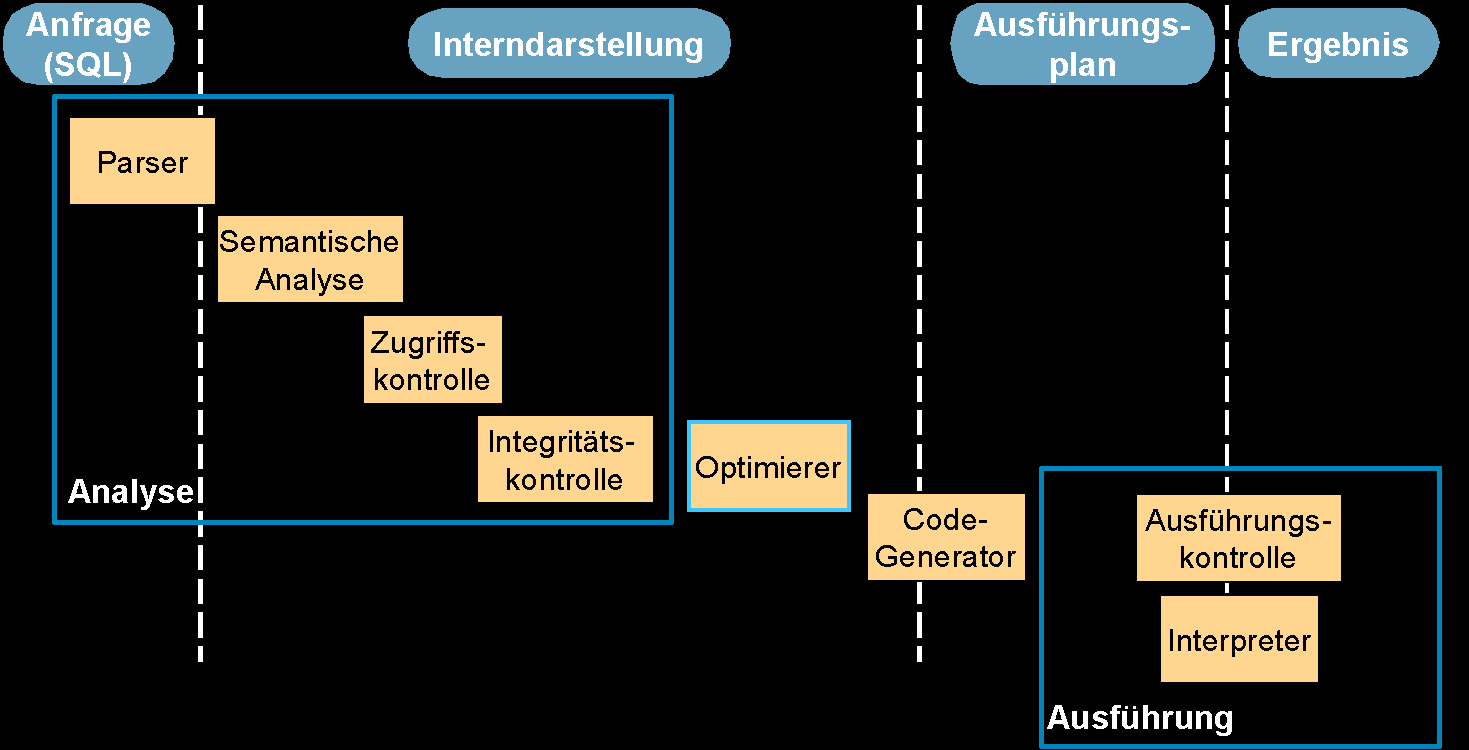
\includegraphics[width=1\linewidth]{Pictures/U10-Beamer-Anfrageverarbeitung}
\pagebreak
\end{beamerText}


\section{Ausführungspläne}
\label{plan}

Gegeben seien folgende Relationen:

\texttt{Employee (\underline{num}, fname, lname, addr, mgr[employee], \beamertxt{\\}dep[department])}

\texttt{Department (\underline{num}, name, mgr[employee])}

\texttt{Project (\underline{num}, dep[department], mgr[employee])}

\texttt{Works\_on (\underline{proj[project], empl[employee]})}

Setzen Sie folgende SQL-Anweisungen in nicht-optimierte Operatorgraphen um. Verwenden Sie dafür die Baum-Notation von Vorlesungsfolie~\Operatorgraph. % stimmt noch (KMW, 04.12.2018)

\fbox{\begin{minipage}{\textwidth}
\paragraph{Hinweis:} Zur weiteren Übung können Sie das Tool DBSnap verwenden: \\
	\DBSnap \\
	Bitte beachten: Es führt bei der Projektion zusätzlich eine Duplikateliminierung durch.

	\begin{note}
		Literatur: Y. N. Silva et al.: DBSnap: Learning Database Queries by Snapping Blocks, SIGCSE 2015, DOI \url{http://dx.doi.org/10.1145/2676723.2677220}
	\end{note}
\end{minipage}}
\begin{enumerate}[a)]

	\item Alle MitarbeiterInnen und ihre Vorgesetzten.
	\begin{lstlisting}
SELECT e.fname, e.lname, s.fname, s.lname
FROM   employee e, employee s
WHERE  e.mgr = s.num
	\end{lstlisting}

\cprotEnv
	\begin{solution}
	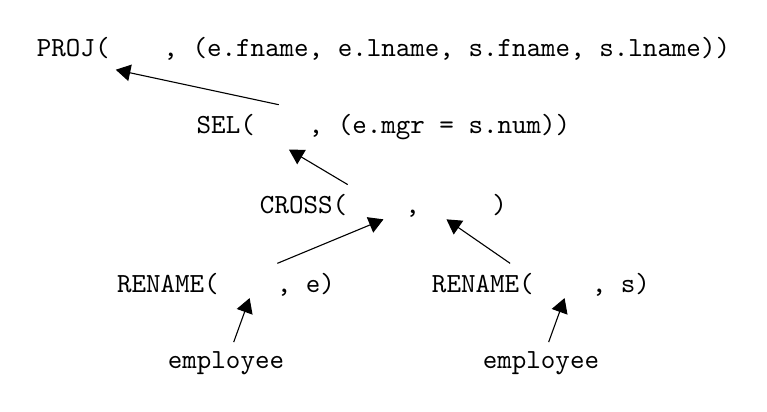
\begin{tikzpicture}
		\node (proj) at(0, 0) {\texttt{PROJ(\hspace{0.5cm} , (e.fname, e.lname, s.fname, s.lname))} };
		\node (sel) [below of =proj] {\texttt{SEL(\hspace{0.5cm} , (e.mgr = s.num))} };
		\node (cross)[below of =sel] {\texttt{CROSS(\qquad, \qquad)} };
		\node (rename1) [below of = cross, xshift=-2cm] {\texttt{RENAME(\qquad, e)}};
		\node (rename2) [below of =cross, xshift=2cm] {\texttt{RENAME(\qquad, s)}};
		\node (emp1) [below of = rename1] {\texttt{employee}};
		\node (emp2) [below of =rename2] {\texttt{employee}};

		\draw[-triangle 60] (sel) -- ($(proj.south) + (-3.4,0)$);
		\draw[-triangle 60] (cross) -- ($(sel.south) + (-1.2,0)$);
		\draw[-triangle 60] (rename1) -- ($(cross.south) + (0.0,0.1)$);
		\draw[-triangle 60] (rename2) -- ($(cross.south) + (0.8,0.1)$);
		\draw[-triangle 60] (emp1) -- ($(rename1.south) + (0.3,0.1)$);
		\draw[-triangle 60] (emp2) -- ($(rename2.south) + (0.3,0.1)$);
	\end{tikzpicture}
\paragraph{\color{solutioncolor}Anmerkung:} In der Tafelübung wird der Einfachheit halber die folgende Darstellung verwendet:
\begin{lstlisting}
- PROJ( , (e.fname, e.lname, s.fname, s.lname))
  - SEL( , (e.mgr = s.num))
    - CROSS( , )
      - RENAME( , e)
        - employee
      - RENAME( , s)
        - employee
\end{lstlisting}
	\end{solution}

\beamertxt{\pagebreak}

	\item Alle MitarbeiterInnen der Forschungsabteilung.
	\begin{lstlisting}
SELECT e.fname, e.lname, e.addr
FROM   employee e
JOIN   department d
ON     d.num = e.dep
WHERE  d.name = 'Research';
	\end{lstlisting}

	\begin{solution}
	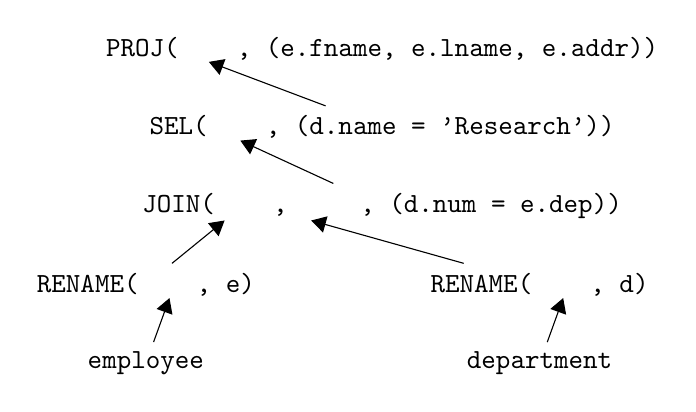
\begin{tikzpicture}
		\node (proj) at (0, 0) {\texttt{PROJ(\qquad , (e.fname, e.lname, e.addr))} };
		\node (sel)[below of =proj] {\texttt{SEL(\qquad , (d.name = 'Research'))} };

		\node (join)[below of =sel] {\texttt{JOIN(\qquad, \qquad, (d.num = e.dep))} };
		\node (renamed)[below of =join, xshift = 2cm] {\texttt{RENAME(\qquad, d)}};
		\node (renamee)[below of =join, xshift =-3cm] {\texttt{RENAME(\qquad, e)}};
		\node (dept)[below of =renamed] {\texttt{department} };
		\node (emp)[below of =renamee] {\texttt{employee} };

		\draw[-triangle 60] (dept) -- ($(renamed.south) + (0.3,0.1)$);
		\draw[-triangle 60] (emp) -- ($(renamee.south) + (0.3,0.1)$);
		\draw[-triangle 60] (renamed) -- ($(join.south) + (-0.9,0.1)$);
		\draw[-triangle 60] (renamee) -- ($(join.south) + (-2,0.1)$);
		\draw[-triangle 60] (join) -- ($(sel.south) + (-1.8,0.1)$);
		\draw[-triangle 60] (sel) -- ($(proj.south) + (-2.2,0.1)$);
	\end{tikzpicture}
	\end{solution}

  \item Alle Abteilungen mit mehr als 10 Mitarbeitern.
	\begin{lstlisting}
SELECT   d.name
FROM     employee e
JOIN     department d
ON       d.num = e.dep
GROUP BY d.num, d.name
HAVING   count(d.num) > 10
	\end{lstlisting}

	\begin{solution}
	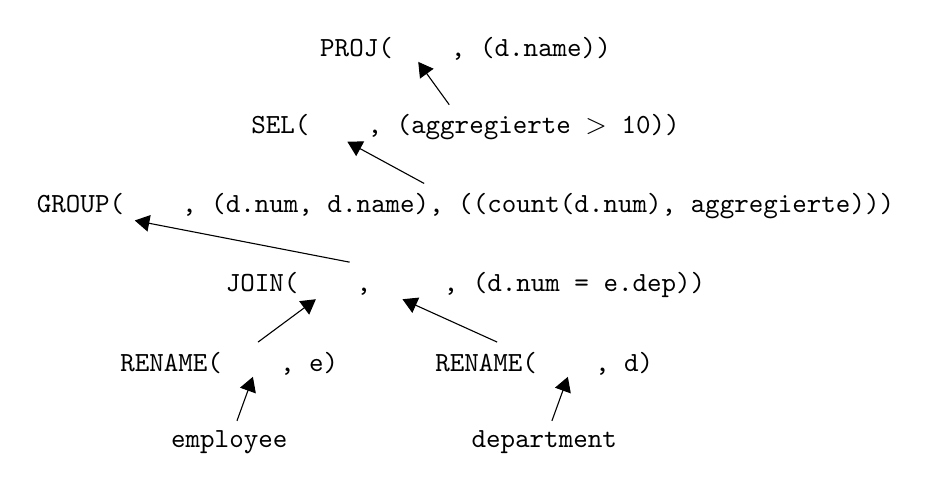
\begin{tikzpicture}
		\node (proj) at (0, 0) {\texttt{PROJ(\qquad , (d.name))} };
		\node (hav)[below of =proj] {\texttt{SEL(\qquad , (aggregierte $>$ 10))} };

		\node (group)[below of =hav] {\texttt{GROUP(\qquad , (d.num, d.name), ((count(d.num), aggregierte)))}};
		\node (join)[below of =group] {\texttt{JOIN(\qquad, \qquad, (d.num = e.dep))} };
		\node (renamed)[below of =join, xshift = 1cm] {\texttt{RENAME(\qquad, d)} };
		\node (renamee)[below of =join, xshift =-3cm] {\texttt{RENAME(\qquad, e)} };
		\node (dept)[below of =renamed] {\texttt{department} };
		\node (emp)[below of =renamee] {\texttt{employee} };

		\draw[-triangle 60] (renamed) -- ($(join.south) + (-0.8,0.1)$);
		\draw[-triangle 60] (renamee) -- ($(join.south) + (-1.9,0.1)$);
		\draw[-triangle 60] (dept) -- ($(renamed.south) + (0.3,0.1)$);
		\draw[-triangle 60] (emp) -- ($(renamee.south) + (0.3,0.1)$);
		\draw[-triangle 60] (join) -- ($(group.south) + (-4.2,0.1)$);
		\draw[-triangle 60] (group) -- ($(hav.south) + (-1.5,0.1)$);
		\draw[-triangle 60] (hav) -- ($(proj.south) + (-0.6,0.1)$);
	\end{tikzpicture}
	\end{solution}

	\item Alle MitarbeiterInnen mit Nachnamen Smith, die eine operative Abteilung leiten oder einem Projekt zugeordnet sind.
	\begin{lstlisting}
SELECT e.lname
FROM ((SELECT p.num, e.lname
    FROM   project p, department d, employee e
    WHERE  d.num = p.dep
    AND    d.mgr = e.num
  )
  UNION
  ( SELECT p.num, e.lname
    FROM   project p, works_on w, employee e
    WHERE  p.num = proj
    AND    e.num = empl
  )
)
WHERE e.lname = 'Smith';
	\end{lstlisting}

	\begin{solution}
	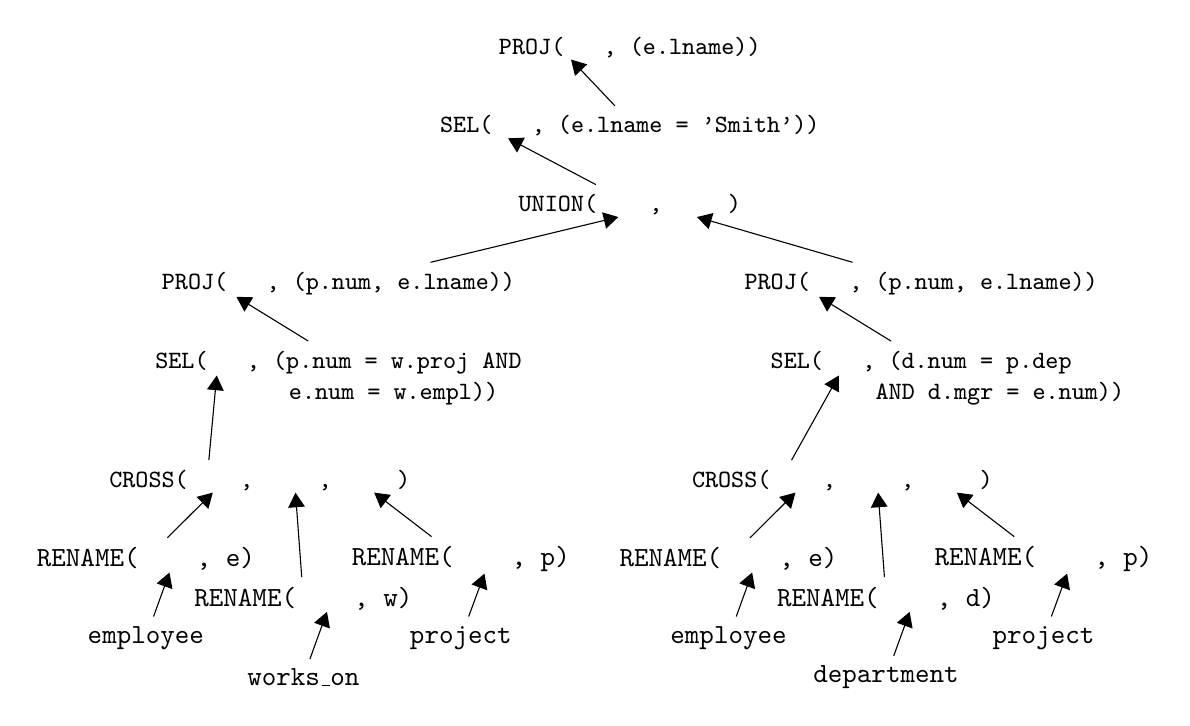
\begin{tikzpicture}
		\node (proj_top) at(0, 0) {\small{\texttt{PROJ(\hspace{0.5cm}, (e.lname))} } };
		\node (sel_top) [below of =proj_top] {\small{\texttt{SEL(\hspace{0.5cm}, (e.lname = 'Smith'))} } };
		\node (union) [below of =sel_top] {\small{\texttt{UNION(\qquad, \qquad)} } };

		\node (proj_left) [below of =union, xshift = 3.7cm] {\small{\texttt{PROJ(\hspace{0.5cm}, (p.num, e.lname))} } };
		\node (proj_right) [below of =union, xshift = -3.7cm] {\small{\texttt{PROJ(\hspace{0.5cm}, (p.num, e.lname))} } };

		\node (sel_left) [below of =proj_left] {\small{\texttt{SEL(\hspace{0.5cm}, (d.num = p.dep} } };
		\node (sel_left2) [below of =sel_left, xshift =1cm, yshift = 0.6cm] {\small{\texttt{AND d.mgr = e.num))} } };
		\node (sel_right) [below of =proj_right, xshift =0cm] {\small{\texttt{SEL(\hspace{0.5cm}, (p.num = w.proj AND} } };
		\node (sel_right2) [below of =sel_right, xshift =0.7cm, yshift = 0.6cm] {\small{\texttt{e.num = w.empl))} } };

		\node (cross_left) [below of =sel_left, xshift =-1cm, yshift =-0.5cm] {\small{\texttt{CROSS(\qquad, \qquad, \qquad)} } };
		\node (cross_right) [below of =sel_right, xshift =-1cm, yshift =-0.5cm] {\small{\texttt{CROSS(\qquad, \qquad, \qquad)} } };

		\node (rename_emp_left) [below of =cross_left, xshift =-1.5cm] {\texttt{RENAME(\qquad, e)}};
		\node (rename_dept_left) [below of =cross_left, xshift =0.5cm, yshift =-0.5cm] {\texttt{RENAME(\qquad, d)} };
		\node (rename_project_left) [below of =cross_left, xshift =2.5cm] {\texttt{RENAME(\qquad, p)}};
		\node (rename_emp_right) [below of =cross_right, xshift =-1.5cm] {\texttt{RENAME(\qquad, e)}};
		\node (rename_works_right) [below of =cross_right, xshift =0.5cm, yshift =-0.5cm] {\texttt{RENAME(\qquad, w)}};
		\node (rename_project_right) [below of =cross_right, xshift =2.5cm] {\texttt{RENAME(\qquad, p)}};

		\node (emp_left) [below of =rename_emp_left] {\texttt{employee} };
		\node (dept_left) [below of =rename_dept_left] {\texttt{department}};
		\node (project_left) [below of =rename_project_left] {\texttt{project} };
		\node (emp_right) [below of =rename_emp_right] {\texttt{employee} };
		\node (works_right) [below of =rename_works_right] {\texttt{works\_on} };
		\node (project_right) [below of =rename_project_right] {\texttt{project} };

		\draw[-triangle 60] (sel_top) -- ($(proj_top.south) + (-0.8,0.1)$);
		\draw[-triangle 60] (union) -- ($(sel_top.south) + (-1.6,0.1)$);

		\draw[-triangle 60] (proj_left) -- ($(union.south) + (0.8, 0.1)$);
		\draw[-triangle 60] (proj_right) -- ($(union.south) + (-0.2, 0.1)$);

		\draw[-triangle 60] (sel_left) -- ($(proj_left.south) + (-1.35,0.1)$);
		\draw[-triangle 60] (sel_right) -- ($(proj_right.south) + (-1.35,0.1)$);

		\draw[-triangle 60] ($(cross_left.north) + (-0.7, 0 )$) -- ($(sel_left.south) + (-1.1,0.1)$);
		\draw[-triangle 60] ($(cross_right.north) + (-0.7, 0 )$) -- ($(sel_right.south) + (-1.6,0.1)$);

		\draw[-triangle 60] (rename_emp_left) -- ($(cross_left.south) + (-0.65,0.1)$);
		\draw[-triangle 60] (rename_dept_left) -- ($(cross_left.south) + (0.4,0.1)$);
		\draw[-triangle 60] (rename_project_left) -- ($(cross_left.south) + (1.4,0.1)$);
		\draw[-triangle 60] (rename_emp_right) -- ($(cross_right.south) + (-0.65,0.1)$);
		\draw[-triangle 60] (rename_works_right) -- ($(cross_right.south) + (0.4,0.1)$);
		\draw[-triangle 60] (rename_project_right) -- ($(cross_right.south) + (1.4,0.1)$);

		\draw[-triangle 60] (emp_left) -- ($(rename_emp_left.south) + (0.3,0.1)$);
		\draw[-triangle 60] (dept_left) -- ($(rename_dept_left.south) + (0.3,0.1)$);
		\draw[-triangle 60] (project_left) -- ($(rename_project_left.south) + (0.3,0.1)$);
		\draw[-triangle 60] (emp_right) -- ($(rename_emp_right.south) + (0.3,0.1)$);
		\draw[-triangle 60] (works_right) -- ($(rename_works_right.south) + (0.3,0.1)$);
		\draw[-triangle 60] (project_right) -- ($(rename_project_right.south) + (0.3,0.1)$);
	\end{tikzpicture}
	\end{solution}

\end{enumerate}


\section{Optimierung}

Optimieren Sie die Ausführungspläne aus Aufgabe~\ref{plan}.
Nutzen Sie dazu die Regeln von Folien~\Operatorregel\ und die Heuristik auf den Folien~\Operatorheuristik.
Die aufgeführten Regeln für die algebraische Umformung sind aber nur Beispiele.
Formulieren Sie offensichtlich mögliche Umformungsmöglichkeiten selbst und nutzen Sie auch diese.

\begin{note}
Beides finden Sie als Referenz noch einmal am Ende dieses Übungsblatts.
\end{note}

\begin{solution}
\begin{enumerate}[a)]

\item Zur Heuristik:

\begin{itemize}
	\item Ausführungsplan beinhaltet nur Selektion mit einem Prädikat-Term $\rightarrow$ keine Separierung notwendig.
	\item Selektion und Kreuzprodukt können zusammengefasst werden (Umformungsregel 9).
\end{itemize}

Das ergibt folgenden optimierten Ausführungsplan:

\begin{center}
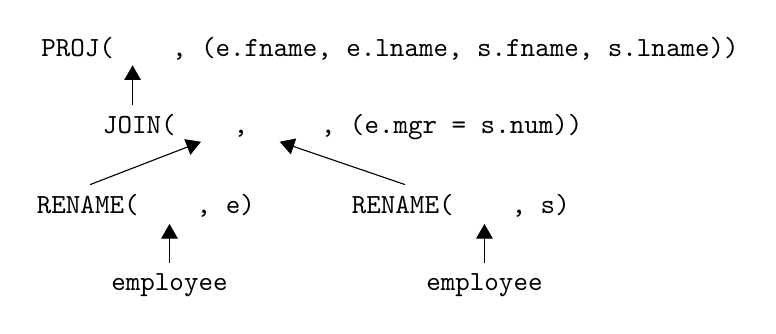
\begin{tikzpicture}
	\node (proj) at(0, 0) {\texttt{PROJ(\qquad, (e.fname, e.lname, s.fname, s.lname))} };
	\node (join) [below of =proj, xshift=-0.6cm] {\texttt{JOIN(\qquad, \qquad, (e.mgr = s.num))} };
	\node (rename_emp1) [below of = join, xshift=-2.5cm] {\texttt{RENAME(\qquad, e)}};
	\node (rename_emp2) [below of =join, xshift=1.5cm] {\texttt{RENAME(\qquad, s)}};
	\node (emp1) [below of = rename_emp1, xshift=0.3cm] {\texttt{employee}};
	\node (emp2) [below of = rename_emp2, xshift=0.3cm] {\texttt{employee}};

	\draw[-triangle 60] ($(rename_emp1.north west) + (0.8,0)$) -- ($(join.south) + (-1.8,0.1)$);
	\draw[-triangle 60] ($(rename_emp2.north west) + (0.8,0)$) -- ($(join.south) + (-0.8,0.1)$);
	\draw[-triangle 60] (emp1.north) -- +(0,0.5);
	\draw[-triangle 60] (emp2.north) -- +(0,0.5);
	\draw[-triangle 60] ($(join.north west) + (0.5,0)$) -- +(0,0.5);
\end{tikzpicture}
\end{center}

\item Die Selektion kann vor den Verbund geschoben werden (Umformungsregel 7).

\begin{center}
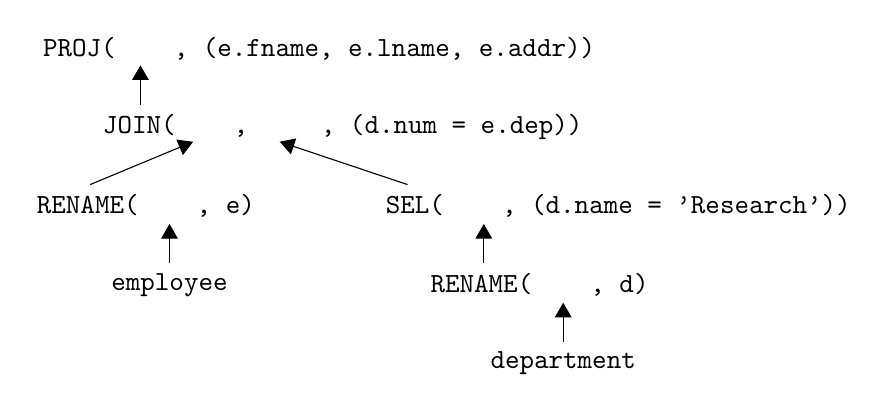
\begin{tikzpicture}
	\node (proj) at(0, 0) {\texttt{PROJ(\qquad, (e.fname, e.lname, e.addr))} };
	\node (join) [below of =proj, xshift=0.3cm] {\texttt{JOIN(\qquad, \qquad, (d.num = e.dep))} };
	\node (r_emp) [below of = join, xshift=-2.5cm] {\texttt{RENAME(\qquad, e)}};
	\node (emp) [below of = r_emp, xshift=0.3cm] {\texttt{employee}};
	\node (sel) [below of =join, xshift=3.5cm] {\texttt{SEL(\qquad, (d.name = 'Research'))} };
	\node (r_dept) [below of = sel, xshift=-1cm] {\texttt{RENAME(\qquad, d)} };
	\node (dept) [below of = r_dept, xshift=0.3cm] {\texttt{department} };

	\draw[-triangle 60] ($(r_dept.north west) + (0.8,0)$) -- +(0,0.5);
	\draw[-triangle 60] ($(r_emp.north west) + (0.8,0)$) -- ($(join.south) + (-1.9,0.1)$);
	\draw[-triangle 60] (dept.north) -- +(0,0.5);
	\draw[-triangle 60] ($(sel.north west) + (0.4,0)$) -- ($(join.south) + (-0.8,0.1)$);
	\draw[-triangle 60] (emp.north) -- +(0,0.5);
	\draw[-triangle 60] ($(join.north west) + (0.6,0)$) -- +(0,0.5);
\end{tikzpicture}
\end{center}

\item Hier kommen wir mit den Heuristiken und Umformungsregeln aus der Vorlesung nicht weiter.
	Da jedoch über den Primärschlüssel vom Department gruppiert wird, die Aggregation nur ein Count umfasst und die Vielfachheit nur aus dem Verbund mit dem Employee stammt, 
	kann man hier die Gruppierung am Join vorbei zum Employee ziehen.

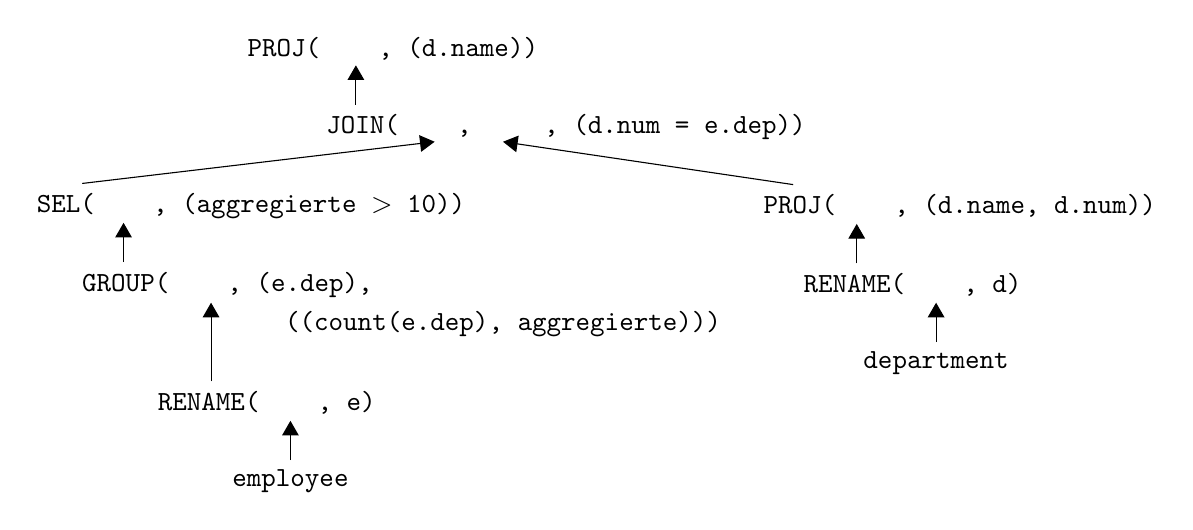
\begin{tikzpicture}
	\node (proj) at (0, 0) {\texttt{PROJ(\qquad , (d.name))} };
	\node (join)[below of =proj, xshift=2.2cm] {\texttt{JOIN(\qquad, \qquad, (d.num = e.dep))} };
	\node (proj2)[below of =join, xshift=5cm] {\texttt{PROJ(\qquad , (d.name, d.num))} };
	\node (hav)[below of =join, xshift=-4cm] {\texttt{SEL(\qquad , (aggregierte $>$ 10))} };
	\node (group)[below of =hav, xshift=-0.3cm] {\texttt{GROUP(\qquad , (e.dep),}};
	\node (group2)[below of =group, xshift=3.5cm, yshift=0.5cm] {\texttt{((count(e.dep), aggregierte)))}};
	\node (renamed)[below of =proj2, xshift=-0.6cm] {\texttt{RENAME(\qquad, d)} };
	\node (renamee)[below of =group, yshift=-0.5cm, xshift =.5cm] {\texttt{RENAME(\qquad, e)} };
	\node (dept)[below of =renamed, xshift=0.3cm] {\texttt{department} };
	\node (emp)[below of =renamee, xshift=0.3cm] {\texttt{employee} };
	
	\draw[-triangle 60] (dept.north) -- +(0,0.5);
	\draw[-triangle 60] (emp.north) -- +(0,0.5);
	\draw[-triangle 60] ($(renamed.north west) + (0.8,0)$) -- +(0,0.5);
	\draw[-triangle 60] ($(renamee.north west) + (0.8,0)$) -- +(0,1);
	\draw[-triangle 60] ($(group.north west) + (0.65,0)$) -- +(0,0.5);
	\draw[-triangle 60] ($(hav.north west) + (0.7,0)$) -- ($(join.south west) + (1.5,0.1)$);
	\draw[-triangle 60] ($(proj2.north west) + (0.5,0)$) -- ($(join.south) + (-0.8,0.1)$);
	\draw[-triangle 60] ($(join.north west) + (0.5,0)$) -- +(0,0.5);

\end{tikzpicture}

\item

\begin{itemize}
	\item Die Selektion "`e.lname = 'Smith'"' kann in beiden Teilbäumen ganz nach unten gezogen werden (Umformungsregeln 6, 7, 8).
	\item Die Selektion und das Kreuzprodukt in den beiden Teilbäumen können jeweils zusammengefasst werden (Umformungsregel 9).
\end{itemize}

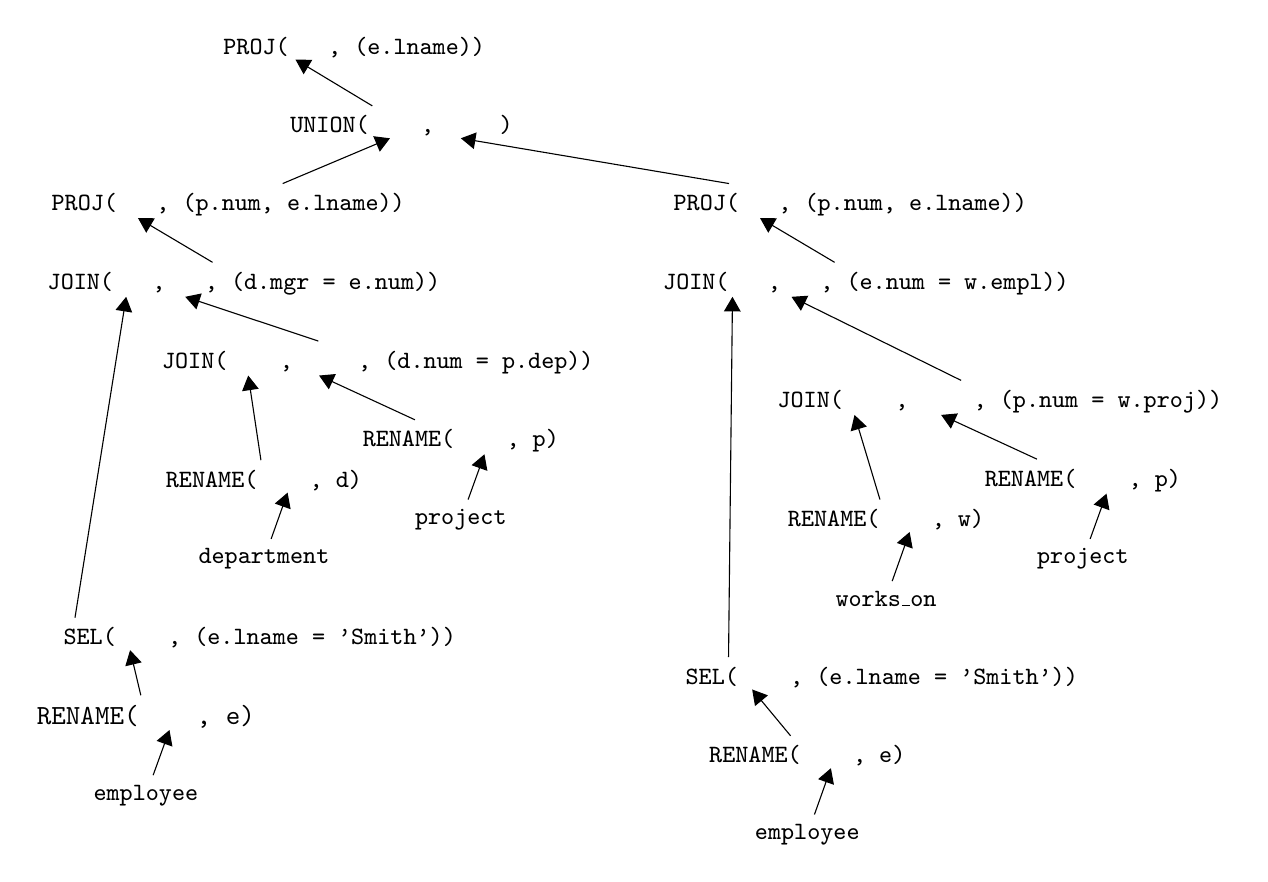
\begin{tikzpicture}
	\node (proj_top) at(0, 0) {\small{\texttt{PROJ(\hspace{0.5cm}, (e.lname))} } };
	\node (union) [below of =proj_top, xshift=0.6cm] {\small{\texttt{UNION(\qquad, \qquad)} } };

	\node (proj_left) [below of =union, xshift =-2.2cm] {\small{\texttt{PROJ(\hspace{0.5cm}, (p.num, e.lname))} } };
	\node (proj_right) [below of =union, xshift =5.7cm] {\small{\texttt{PROJ(\hspace{0.5cm}, (p.num, e.lname))} } };

	\node (join_left1) [below of =proj_left, xshift =0.2cm]  {\small{\texttt{JOIN(\hspace{0.5cm},\hspace{0.5cm}, (d.mgr = e.num))} } };
	\node (join_right1) [below of =proj_right, xshift =0.2cm] {\small{\texttt{JOIN(\hspace{0.5cm},\hspace{0.5cm}, (e.num = w.empl))} } };

	\node (join_left2) [below of =join_left1, xshift =1.7cm] {\small{\texttt{JOIN(\qquad, \qquad, (d.num = p.dep))} } };
	\node (join_right2) [below of =join_right1, xshift =1.7cm, yshift=-0.5cm] {\small{\texttt{JOIN(\qquad, \qquad, (p.num = w.proj))} } };

	\node (rename_dept_left) [below of =join_left2, xshift =-1.5cm, yshift=-0.5cm] {\small\texttt{RENAME(\qquad, d)} };
	\node (dept_left) [below of =rename_dept_left] {\small\texttt{department}};
	\node (rename_project_left) [below of =join_left2, xshift =1cm] {\small\texttt{RENAME(\qquad, p)}};
	\node (project_left) [below of =rename_project_left] {\small\texttt{project} };

	\node (rename_works_right) [below of =join_right2, xshift =-1.5cm, yshift =-0.5cm] {\small\texttt{RENAME(\qquad, w)}};
	\node (works_right) [below of =rename_works_right] {\small\texttt{works\_on} };
	\node (rename_project_right) [below of =join_right2, xshift =1cm] {\small\texttt{RENAME(\qquad, p)}};
	\node (project_right) [below of =rename_project_right] {\small\texttt{project} };


	\node (sel_left) [below of =dept_left, xshift =0cm] {\small{\texttt{SEL(\qquad, (e.lname = 'Smith'))} } };
	\node (sel_right) [below of =works_right, xshift =0cm] {\small{\texttt{SEL(\qquad, (e.lname = 'Smith'))} } };

	\node (rename_emp_left) [below of =sel_left, xshift =-1.5cm] {\texttt{RENAME(\qquad, e)}};
	\node (emp_left) [below of =rename_emp_left] {\small\texttt{employee} };
	\node (rename_emp_right) [below of =sel_right, xshift =-1cm] {\small\texttt{RENAME(\qquad, e)}};
	\node (emp_right) [below of =rename_emp_right] {\small\texttt{employee} };

	\draw[-triangle 60] (union) -- ($(proj_top.south) + (-0.8,0.1)$);
	\draw[-triangle 60] (proj_left) -- ($(union.south) + (-0.2,0.1)$);
	\draw[-triangle 60] (proj_right) -- ($(union.south) + (0.7,0.1)$);

	\draw[-triangle 60] (join_left1) -- ($(proj_left.south) + (-1.2,0.1)$);
	\draw[-triangle 60] (join_right1) -- ($(proj_right.south) + (-1.2,0.1)$);

	\draw[-triangle 60] (join_left2) -- ($(join_left1.south) + (-0.8,0.1)$);
	\draw[-triangle 60] (join_right2) -- ($(join_right1.south) + (-1,0.1)$);

	\draw[-triangle 60] (rename_dept_left) -- ($(join_left2.south) + (-1.7,0.1)$);
	\draw[-triangle 60] (rename_project_left) -- ($(join_left2.south) + (-0.8,0.1)$);

	\draw[-triangle 60] (rename_works_right) -- ($(join_right2.south) + (-1.9,0.1)$);
	\draw[-triangle 60] (rename_project_right) -- ($(join_right2.south) + (-0.8,0.1)$);

	\draw[-triangle 60] ($(sel_left.north) + (-2.4, 0 )$) -- ($(join_left1.south) + (-1.55,0.1)$);
	\draw[-triangle 60] ($(sel_right.north) + (-2, 0 )$) -- ($(join_right1.south) + (-1.75,0.1)$);

	\draw[-triangle 60] (rename_emp_left) -- ($(sel_left.south) + (-1.7,0.1)$);
	\draw[-triangle 60] (rename_emp_right) -- ($(sel_right.south) + (-1.7,0.1)$);
	\draw[-triangle 60] (emp_left) -- ($(rename_emp_left.south) + (0.3,0.1)$);
	\draw[-triangle 60] (dept_left) -- ($(rename_dept_left.south) + (0.3,0.1)$);
	\draw[-triangle 60] (project_left) -- ($(rename_project_left.south) + (0.3,0.1)$);
	\draw[-triangle 60] (emp_right) -- ($(rename_emp_right.south) + (0.3,0.1)$);
	\draw[-triangle 60] (works_right) -- ($(rename_works_right.south) + (0.3,0.1)$);
	\draw[-triangle 60] (project_right) -- ($(rename_project_right.south) + (0.3,0.1)$);
	\end{tikzpicture}

\paragraph{\color{solutioncolor}Ergänzung:}
In der Literatur ist es üblich, Operatoren mit griechischen Buchstaben darzustellen.
Diese Darstellung sollte vor allem den Lehramtsstudierenden bekannt sein.
Der eben erstellte Baum würde dann folgendermaßen aussehen:

\begin{center}
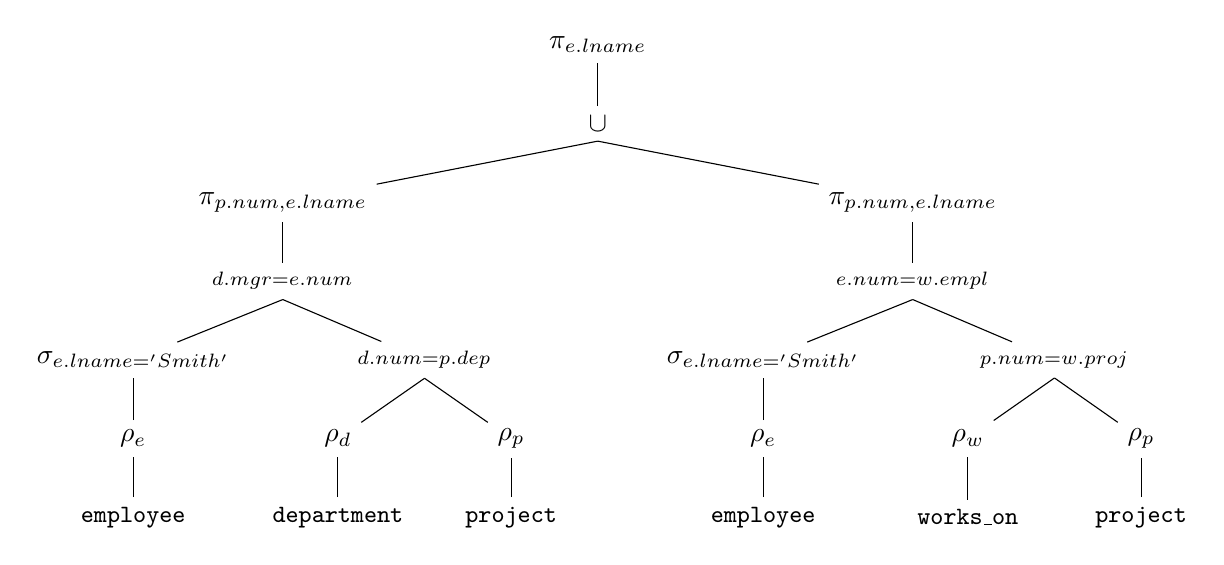
\begin{tikzpicture}
    \node (proj_top) at(0, 0) {$\pi_{\text{e.lname}}$ };
    \node (union) [below of =proj_top] {$\cup$} ;

    \node (proj_left) [below of =union, xshift =-4.0cm] {$\pi_{\text{p.num, e.lname}}$ };
    \node (proj_right) [below of =union, xshift =4.0cm] {$\pi_{\text{p.num, e.lname}}$ };

    \node (join2_left) [below of =proj_left] {$\Bowtie_{\text{d.mgr = e.num}}$};
    \node (join2_right) [below of =proj_right] {$\Bowtie_{\text{e.num = w.empl}}$};

    \node (sel_left) [below of =join2_left, xshift = -1.9cm] {$\sigma_{\text{e.lname = 'Smith'}}$};
    \node (sel_right) [below of =join2_right, xshift = -1.9cm] {$\sigma_{\text{e.lname = 'Smith'}}$};

    \node (join1_left) [below of =join2_left, xshift = 1.8cm] {$\Bowtie_{\text{d.num = p.dep}}$};
    \node (r_dep_left) [below of =join1_left,xshift = -1.1cm] {$\rho_{\text{d}}$};
    \node (r_project_left) [below of =join1_left,xshift = 1.1cm] {$\rho_{\text{p}}$};
    \node (r_emp_left) [below of =sel_left] {$\rho_{\text{e}}$};
    \node (dep_left) [below of =r_dep_left] {\small{\texttt{department}}};
    \node (project_left) [below of =r_project_left] {\small{\texttt{project}}};
    \node (emp_left) [below of =r_emp_left] {\small{\texttt{employee}}};

    \node (join1_right) [below of =join2_right, xshift = 1.8cm] {$\Bowtie_{\text{p.num = w.proj}}$};
    \node (r_works_right) [below of =join1_right,xshift = -1.1cm] {$\rho_{\text{w}}$};
    \node (r_project_right) [below of =join1_right,xshift = 1.1cm] {$\rho_{\text{p}}$};
    \node (r_emp_right) [below of =sel_right] {$\rho_{\text{e}}$};
    \node (works_right) [below of =r_works_right] {\small{\texttt{works\_on}}};
    \node (project_right) [below of =r_project_right] {\small{\texttt{project}}};
    \node (emp_right) [below of =r_emp_right] {\small{\texttt{employee}}};

    \draw (r_emp_left) -- ($(sel_left.south)$);
    \draw (emp_left) -- ($(r_emp_left.south)$);
    \draw (sel_left) -- ($(join2_left.south)$);
    \draw (join2_left) -- ($(proj_left.south)$);
    \draw (proj_left) -- ($(union.south)$);

    \draw (r_dep_left) -- ($(join1_left.south)$);
    \draw (r_project_left) -- ($(join1_left.south)$);
    \draw (dep_left) -- ($(r_dep_left.south)$);
    \draw (project_left) -- ($(r_project_left.south)$);
    \draw (join1_left) -- ($(join2_left.south)$);

    \draw (r_emp_right) -- ($(sel_right.south)$);
    \draw (emp_right) -- ($(r_emp_right.south)$);
    \draw (sel_right) -- ($(join2_right.south)$);
    \draw (join2_right) -- ($(proj_right.south)$);
    \draw (proj_right) -- ($(union.south)$);

    \draw (r_works_right) -- ($(join1_right.south)$);
    \draw (r_project_right) -- ($(join1_right.south)$);
    \draw (works_right) -- ($(r_works_right.south)$);
    \draw (project_right) -- ($(r_project_right.south)$);
    \draw (join1_right) -- ($(join2_right.south)$);

    \draw (union) -- ($(proj_top.south)$);
\end{tikzpicture}
\end{center}

\end{enumerate}
\end{solution}

\begin{note}
    Anmerkung: Diese Darstellung könnte vor allem für Lehramtsstudierende wichtig sein,
    da sie prinzipiell im Staatsexamen erwartet werden kann.
\end{note}


\beamertxt{\pagebreak}
\begin{deeper}
\section{Ausführungspläne und Optimierung 2}

Gegeben sind folgende aus Aufgabe \ref{plan} bekannte Relationen:

\texttt{Employee (\underline{num}, fname, lname, addr, mgr[employee], dep[department])}

\texttt{Department (\underline{num}, name, mgr[employee])}

\texttt{Project (\underline{num}, dep[department], mgr[employee])}

\texttt{Works\_on (\underline{proj[project], empl[employee]})}

Setzen Sie die folgenden SQL-Anweisungen in nicht-optimierte Operatorgraphen um.
Verwenden Sie dafür die Baum-Notation von Vorlesungsfolie~\Operatorgraph.
Optimieren Sie die Anweisungen anschließend und zeichnen Sie jeweils den optimierten Operatorgraph.

\cprotEnv
\begin{normalText}
\begin{enumerate}[a)]
	\item
\begin{lstlisting}
-- Alle MitarbeiterInnen mit Vorgesetzten in anderen
-- Departments
SELECT e.fname, e.lname
FROM   employee e, employee s
WHERE  e.mgr = s.num
AND    NOT e.dep = s.dep
\end{lstlisting}

\cprotEnv
\begin{note}
Nicht optimiert:
\begin{lstlisting}
- PROJ( , (e.fname, e.lname))
  - SEL( , (e.mgr = s.num AND NOT e.dep = s.dep))
    - CROSS(employee e, employee s)
\end{lstlisting}
Optimiert:
\begin{lstlisting}
- PROJ( , (e.fname, e.lname))
  - JOIN( , ,  (e.mgr = s.num AND NOT e.dep = s.dep))
    - employee e
    - employee s
\end{lstlisting}
Regel 9
\end{note}

\item

\begin{lstlisting}
-- Alle Vorgesetzen, die ein Department leiten, zu dem sie
-- nicht selbst gehoeren
SELECT   s.fname, s.lname
FROM     employee s
JOIN     department d
ON       d.mgr = s.num
JOIN     employee e
ON       e.mgr = s.num
WHERE    NOT d.num = s.dep
GROUP BY s.fname, s.lname, s.num
\end{lstlisting}
\cprotEnv
\begin{note}
Nicht optimiert:
\begin{lstlisting}
-PROJ( , (s.fname, s.lname))
  -GROUP( , (s.fname, s.lname, s.num))
    -SEL( , (NOT d.num = s.dep))
      -JOIN(employee e, , (e.mgr = s.num))
        -JOIN(employee s, department d, (d.mgr = s.num))
\end{lstlisting}
  Optimiert: Sel durch äußeren Join ziehen, dann Sel und Join verschmelzen.
  e vor dem Join auf mgr projizieren.\\
\begin{lstlisting}
-PROJ( , (s.fname, s.lname))
  -GROUP( , (s.fname, s.lname, s.num))
    -JOIN( , (e.mgr = s.num))
      -PROJ(employee e, (e.mgr))
      -JOIN( , , (d.mgr = s.num AND NOT d.num = s.dep))
        -employee s
        -department d

\end{lstlisting}
Regeln 1, 7, 9, 4, 9, 6
\end{note}

\item

	\begin{lstlisting}
-- Pro Department die durchschnittliche Anzahl der
-- Mitarbeiter der von diesem Department durchgefuehrten
-- Projekte fuer Departments, die von einem Mitarbeiter
-- mit Nachnamen Smith geleitet werden
SELECT   AVG(a.anzahl) as durchschnitt, d.name
FROM     (
          SELECT   count(*) as anzahl, proj
          FROM     works_on
          GROUP BY proj
         ) a
JOIN     project p
ON       a.proj = p.num
JOIN     department d
ON       d.num = p.dep
JOIN     employee m
ON       m.num = d.mgr
GROUP BY m.lname, d.num, d.name
HAVING   m.lname = 'Smith'
	\end{lstlisting}

\begin{note}
	Nicht optimiert:
	\begin{equation*}
\begin{split}
	 & \pi_{durchschnitt, d.name}( \quad )                                                     \\
	 & \quad \sigma_{m.lname = 'Smith'}(\quad)                                                 \\
	 & \qquad \gamma_{(m.lname, d.num, d.name), avg(a.anzahl) \rightarrow durchschnitt}(\quad) \\
	 & \qquad\quad \underset{a.proj = p.num}{\bowtie}                                          \\
	 & \qquad \quad  \underset{d.num = p.dep}{\bowtie}                                         \\
	 & \qquad \quad \underset{m.num = d.mgr}{\bowtie}                                          \\
	 & \qquad\qquad \rho_{a}(\pi_{anzahl, proj}(\quad )                                        \\
	 & \qquad\qquad\quad\gamma_{(proj), count(*) \rightarrow anzahl}(works\_on))               \\
	 & \qquad\qquad \rho_{p}(project)                                                          \\
	 & \qquad\qquad \rho_{d}(department)                                                       \\
	 & \qquad\qquad \rho_{m}(employee)
\end{split}
\end{equation*}

Optimierungen: Sicherlich vieles möglich, offensichtlich: HAVING durch GROUP ziehen, GROUP um lname kürzen.
\end{note}
\end{enumerate}
\end{normalText}

\end{deeper}

\beamertxt{\pagebreak}
\section{Relationale Algebra}

Gegeben seien die Relationen R und S. Gilt die folgende Behauptung? Begründen Sie Ihre Antwort!

\texttt{PROJ(INTERSECT(R, S), E) = \beamertxt{\\ \hspace*{3em} =} INTERSECT(PROJ(R, E), PROJ(S, E))}

Umgangssprachlich: Dürfen Projektion und Schnittmenge vertauscht werden?

\begin{solution}
Die Behauptung gilt nicht.

Ein Gegenbeispiel: Gegeben seien die Relationen R und S:
\begin{center}
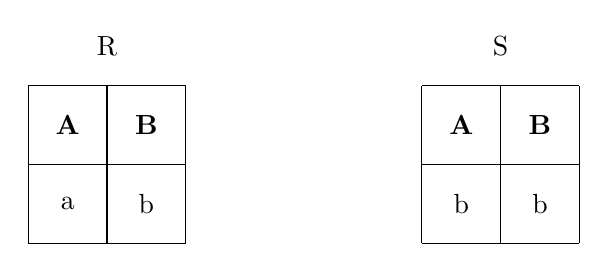
\begin{tikzpicture}
	\draw (0, 0) grid+(2, 2)
				(5, 0) grid+(2, 2);

	\node at(1, 2.5) {R};
	\node at(0.5, 0.5) {a};
	\node at(0.5, 1.5) {\textbf{A}};
	\node at(1.5, 0.5) {b};
	\node at(1.5, 1.5) {\textbf{B}};

	\node at(6, 2.5) {S};
	\node at(5.5, 0.5) {b};
	\node at(5.5, 1.5) {\textbf{A}};
	\node at(6.5, 0.5) {b};
	\node at(6.5, 1.5) {\textbf{B}};
\end{tikzpicture}
\end{center}

\texttt{PROJ(INTERSECT(R, S), B) = \{\}}, weil schon \texttt{INTERSECT(R, S) = \{\} }

Aber:
\texttt{INTERSECT(PROJ(R, B), PROJ(S, B)) = \{[b]\} }
\end{solution}

\begin{note}

\section*{Referenz: Vorlesungsfolien}

\paragraph{Hinweis:} Diese Umformungsregeln und Heuristiken werden in der Klausur \emph{nicht} angegeben.

\subsection*{Umformungsregeln}

\begin{enumerate}
	\item Ein n-facher Verbund kann durch eine Folge von binären Verbunden ersetzt werden und umgekehrt.
	\item Verbund ist kommutativ.
	\item Verbund ist assoziativ.
	\item Selektionen können zusammengefasst werden: \\
	\texttt{SEL(SEL(R,pred1),pred2) = SEL(R,(pred1 AND pred2))}
	\item Projektionen können zusammengefasst werden: \\
	\texttt{PROJ(PROJ(R,L1),L2) = PROJ(R,L2)}
	\item Projektion dürfen (in erweiterter Form) vorgezogen werden: \\
	\texttt{PROJ(SEL(R,pred(M)),L) = PROJ(SEL(PROJ(R,(L $\cup$ M)),pred(M)),L)}
	\item Selektion und Verbund dürfen vertauscht werden: \\
	\texttt{SEL(JOIN(R,S,pred1),pred2(R)) = JOIN(SEL(R,pred2),S,pred1)}
	\item Selektion darf mit Vereinigung und Differenz vertauscht werden: \\
	\texttt{SEL(UNION(R,S),pred) = UNION(SEL(R,pred),SEL(S,pred))}
	\item Selektion und Kreuzprodukt können zu Verbund zusammengefasst werden: \\
	\texttt{SEL(CROSS(R,S),pred) = JOIN(R,S,pred)}
\end{enumerate}


\subsection*{Heuristik zur Umformung}

\begin{itemize}
	\item \textbf{Komplexe Verbundoperationen zerlegen} in binäre Verbunde (Bilden von binären Verbunden)
	\item \textbf{Selektionen mit mehreren Prädikat-Termen separieren} in Selektionen mit jeweils einem Prädikat-Term
	\item \textbf{Selektionen so früh wie möglich ausführen}, d.\,h.\ Selektionen hinunterschieben zu den Blättern des Anfragegraphen (engl.\ selection push-down)
	\item \textbf{Selektionen und Kreuzprodukt zu Verbund zusammenfassen}, wenn das Selektionsprädikat Attribute aus den beiden Relationen verwendet
	\item \textbf{Einfache Selektionen wieder zusammenfassen}, d.\,h.\ aufeinanderfolgende Selektionen (derselben Relation) gruppieren
	\item \textbf{Projektionen so früh wie möglich ausführen}, d.\,h.\ Projektionen hinunterschieben zu den Blättern des Anfragegraphen, allerdings nicht vor die Selektion (engl.\ projection push-down); dabei aber die teure Duplikateliminierung vermeiden!
\end{itemize}
\pagebreak
\end{note}


\beamertxt{\pagebreak}
\begin{deeper}
\section{Programmieraufgabe 7: Planoperatoren}

\subsection{Aufgabenstellung}
\begin{enumerate}
	\item Implementieren Sie 6 Klassen, die die Schnittstelle \beamertxt{\linebreak}\texttt{idb.module.Module} implementieren.
		Beachten Sie die Dokumentation der Methoden in der Schnittstelle.
		Diese 6 Klassen entsprechen den Planoperatoren \textit{Projektion, Rename, Selektion, Kreuzprodukt, OrderBy, Table Scan}.
		Nutzen Sie für alle Planoperatoren, die Daten aus einem anderen Operator erhalten, ein \texttt{idb.module.Module} als Quelle dieser Daten, wie auch in den entsprechenden Methoden in \texttt{idb.construct.Util} vorgesehen.
		Bei dem Kreuzprodukt entsprechen die beiden Strings Präfixe für den Namen der jeweiligen Seite. \texttt{leftS} kann auch auf \texttt{null} gesetzt werden um Vielfachkreuzprodukte umsetzen zu können. In diesem Fall werden Attributnamen aus dieser Seite ohne Präfix übernommen.
		Für OrderBy ist ein Komparator bereits in \texttt{idb.module.Util} gegeben. Die Syntax \texttt{String... arg} entspricht auf der Callee-Seite einem Array und ist damit mit dem Parameter in \texttt{idb.module.Util} ausgelegt.
		Achten Sie bei OrderBy darauf, das nächste Element im \texttt{pull()} mit Bubblesort in \textit{O(n)} zu finden.
		Implementieren Sie keinen anderen (Pufferlastigeren) Sortieralgorithmus.
		Tragen Sie die entsprechenden Konstruktoren in \texttt{idb.construct.Util} ein.
	\item Implementieren Sie zusätzlich unter \textit{Store} einen Planoperator, der eine \linebreak \texttt{idb.record.SeqRecordFile} nutzt, um alle Daten des darin eingebauten Operators beim ersten \texttt{pull()} in eine neu angelegte Datei zu speichern und ab dann diese auszulesen. Achten Sie darauf, diese Datei mit \texttt{java.io.File.createTempFile} anzulegen und im \texttt{close} wieder zu löschen.
		Tragen Sie den entsprechenden Konstruktor in \texttt{idb.construct.Util} ein.
	\item Implementieren Sie außerdem unter \textit{Generate} einen Planoperator, mit dessen Hilfe weitere Attribut-Wert Kombinationen (als \texttt{NamedCombinedRecord}) zu den bereits enthaltenen Informationen erzeugt werden können (z.B. bei der Berechnung und Filterung von Strings nach ihrer Länge). Die von der übergebenen Funktion zurückgegebene \texttt{NamedCombinedRecord} sind als Zusätze und nicht als Ersatz der Tupel zu sehen (Hinweis: \texttt{NamedCombinedRecord::combine}).
		Tragen Sie den entsprechenden Konstruktor in \texttt{idb.construct.Util} ein.
	\item Implementieren Sie die Funktion \texttt{idb.construct.Util.delete}, mit deren Hilfe Daten aus einer TID-File gelöscht werden sollen.
		Achten Sie darauf, alle Module ordnungsgemäß zu schließen.
		Bei einer eventuell auftretenden Exception muss Ihre Datenbank sich nicht korrekt verhalten.
	\item Implementieren Sie abschließend \textit{GroupBy} mit Verwendung der bereits existierenden \textit{OrderBy, Projektion}. \texttt{String ...vars} geht dabei direkt in den \textit{OrderBy} über (mittels \texttt{generateOrder(/*TODO*/, /*TODO*/, vars)}).
		\texttt{funcs} entspricht dabei den Aggregationsfunktionen für die Gruppierung.
		Dabei entspricht jeder Eintrag in dieser Liste einer Aggregierung (z.B. \textit{max(MatrNr)}).
		Das Tripel besteht aus den folgenden drei Teilen:
		\begin{enumerate}
			\item Initialer Wert als \texttt{NamedCombinedRecord} für eine leere Gruppierung.
			\item Name des neu erzeugten Attributes als String.
			\item Funktion um aus zwei (Zwischen-)werten einen gemeinsamen Wert zu bilden. (z.B. bei Count: sowas wie \texttt{return a + b}, jedoch für NamedCombinedRecord).
		\end{enumerate}
		Zur Erzeugung dieser Tripels gibt es \texttt{count}, \texttt{min}, \texttt{max} in \texttt{idb.construct.Util}.
		\textit{Seitenbemerkung, für Interessierte: Diese Darstellung von Funktionen funktioniert nur für eine reduzierte Menge an Funktionen wie count, max, min, sum.
		Für avg ist sie ungeeignet, avg muss über die Eigenschaft sum/count umgesetzt werden.}
		Tragen Sie den entsprechenden Konstruktor in \texttt{idb.construct.Util} ein.
	\item Sorgen Sie dafür, dass Sie alle Tests aus den Klassen in \texttt{tests/ProjTests} erfüllen.
	Sie können diese Testfälle mit \lstinline|ant Meilenstein7| ausführen.
	Die einzelnen Unterpunkte hier lassen sich mit \lstinline|ant Meilenstein7a| bis \lstinline |ant Meilenstein7e| ausführen (mit Ausnahme von \lstinline|ant Meilenstein7b|, der nur durch \lstinline|ant Meilenstein 7d| abgedeckt wird).
	Sollten diese Meilensteine 7a bis 7e fehlen, aktualisieren Sie bitte Ihre Version auf die aktualisierten Build-Files der Angabe.
	\item Achten Sie bei allen Modulen darauf, dass die Konstruktion günstig ist und nicht schon \texttt{pull, read} oder ähnliche Funktionen aufruft.
		Sollten Sie Daten haben, die durch einen Aufruf dieser Funktionen initialisiert werden würden, markieren Sie sich den Zustand als unbearbeitet und führen Sie entsprechende Initialisierungen erst beim ersten \texttt{pull} aus.
	\item Die Abgabe auf GitLab erfolgt zeitgleich mit der Abgabe der Zusatzaufgaben des nächsten Übungsblattes auf StudOn. Markieren Sie hierfür Ihre Abgabe mit dem Tag "`Aufgabe-7"'.
\end{enumerate}

\end{deeper}

% \begin{solution}

\section{Implementierung eines Hash-Index}

Aufgabenstellung: Siehe Blatt 7.

\end{solution}


\lstset{basicstyle=\ttfamily,language=C}

\begin{solution}

\begin{algorithm}[H]
\caption{get(key): Gib alle Werte für den gegebenen Schlüssel zurück}
values = \{\}\;
segmentNo = PRIMARY\_SEGMENT\;
pageNo = computeHash(key)\;
\While{pageNo $\neq$ \textbf{undef}}{
	page = fix(segmentNo, pageNo)\;
	values = values $\cup$ extractValues(page, key)\;
	ofPageNo = getOverflowPointer(page)\;
	unfix(segmentNo, pageNo)\;
	segmentNo = OVERFLOW\_SEGMENT\;
	pageNo = ofPageNo\;
}
\Return values\;
\end{algorithm}
\pagebreak[0]

\begin{algorithm}[H]
\caption{put(key, value): Füge neues Schlüssel-Wert-Paar in den Index ein}

segment = PRIMARY\_SEGMENT\;
pageNo = computeHash(key)\;
\For{true}{
	page = fix(segmentNo, pageNo)\;
	numberOfEntries = extractNoE(page)\;
	\eIf{numberOfEntries $<$ BFR}{
		insertItem(page, key, value)\;
		setDirty(segmentNo, pageNo)\;
		unfix(segmentNo, pageNo)\;
		\textbf{break}\;
	}{
		ofPageNo = getOverflowPointer(page)\;
		\If{ofPageNo == \textbf{undef}}{
			ofPageNo = addOverflowBucket()\;
			setOverflowPointer(page, ofPageNo)\;
			setDirty(segmentNo, pageNo)\;
		}
		unfix(segmentNo, pageNo)\;
		segmentNo = OVERFLOW\_SEGMENT\;
		pageNo = ofPageNo\;
	}
}
NUM\_ITEMS = NUM\_ITEMS + 1\;
\If{NUM\_ITEMS /((CAPACITY + POSITION) * BFR) $>$ THRESHOLD}{
	split()\;
}
\end{algorithm}
\pagebreak[0]
\begin{algorithm}[H]
\caption{computeHash(key)}
hash = abs(hashValue(key) $\bmod$ CAPACITY)\;
\If{hash $<$ POSITION}{
	hash = abs(hashValue(key) $\bmod$ (CAPACITY * 2))\;
}
\Return hash\;
\end{algorithm}
\pagebreak[0]
\begin{algorithm}[H]
\caption{split()}
addPrimaryBucket()\;
oldPosition = POSITION\;
POSITION = POSITION + 1\;
\If{POSITION == CAPACITY}{
	POSITION = 0\;
	CAPACITY = CAPACITY * 2\;
}
segmentNo = PRIMARY\_SEGMENT\;
pageNo = oldPosition\;
\While{pageNo $\neq$ \textbf{undef}}{
	page = fix(segmentNo, pageNo)\;
	\ForAll{(key, value) $\in$ page}{
		removeItem(page, (key, value))\;
		setDirty(segmentNo, pageNo)\;
		put(key, value)\;
	}
	ofPageNo = getOverflowPointer(page)\;
	unfix(segmentNo, pageNo)\;
	segmentNo = OVERFLOW\_SEGMENT\;
	pageNo = ofPageNo\;
}
\end{algorithm}
\end{solution}


\end{document}
